\begin{center}
    \vspace*{1.5cm}
    {\fontsize{20}{20}\textbf{\fontspec{Lucida Sans Unicode}Skånska visor}}\\
    \vspace{0.7cm}
    {\fontsize{12}{12}\textit{Om gåsapågen själv får välja}}
\end{center}
\addtocwithheader{Skånska visor}  % Add entry to TOC and set header\noBackground
\noBackground

\newpage
\resetBackground



\subsection*{Skånsk ordlista}

Om du inte kommer från Skåne och nyss flyttat hit för att plugga på LTH, 
kan det ibland vara svårt att förstå alla ord som sägs. Då kan det vara bra
med en Skånsk ordlista. \\



Mög - Skit

Rullebör - Skottkärra

Hutta - Kasta

Räligt - Äckligt

Hem om - Att åka förbi hem innan man åker någonstans

Fubbick - Idiot

Hialös - Jäktad, rastlös

Påg - Pojke

Tös, tösabid - Flicka

Päror - Potatis

Glytting - Barnslig

Klyddigt - Besvärligt

Klydderöv - Krånglig person

Skula - Att ta skydd mot regn

Prega - Att pressa/trycka

Sulten - Mycket hungrig

Läbbigt - Läskigt

Redig - Ordentlig

Blannevann - Groggvirke

Flabben - Käften/munnen

Hossor - Strumpor

Ålahue - Korkad person

Puligt - Najs

\newpage


\subsection*{Vi klarar oss nog ändå} 
\index[alfa]{Vi klarar oss nog ändå}
\index[anfa]{Jag vill sjunga en visa i klaraste dur}
\songinfo{Text: Lasse Dahlquist\\Sång: Edvard Persson}

\begin{parse lines}[\noindent]{#1\\}
    Jag vill sjunga en visa i klaraste dur,
    ty den handlar om Skåne och slätter och djur
    Kan hända den retar en del 
    men i så fall är det deras eget fel
    Det har talats så mycket om dynga och lort 
    men betänk vilken oerhörd nytta den gjort
    ||: Så låt dem bara gå på, vi klarar oss nog ändå :||
    % Ja låt dom bara gå på vi klarar oss nog ändå

    Kanske språket vi talar ej klingar så väl,
    men det är och förbliver en del av vår själ
    Kan hända det retar en del,
    men i så fall är det deras eget fel
    Uti självaste riksda'n på skånska dom slåss,
    för de flesta utav dom har kommit från oss
    ||: Så låt dem... :||
    % Så låt dom bara gå på...

    Utav våra produkter de smörjer sitt krås,
    och de är ifrån oss som dom fått Mårten Gås
    Kan hända det retar en del,
    men i så fall är det deras eget fel
    Det har klagats på bostaden på våra svin
    men när julskinkan kommer jo då är den fin
    ||: Så låt dem... :||
    % Så låt dom bara gå på...
\end{parse lines}

\newpage
\noBackground
% \begin{textblock*}{3cm}(4.0cm,8.0cm) % {width}(x, y)
%     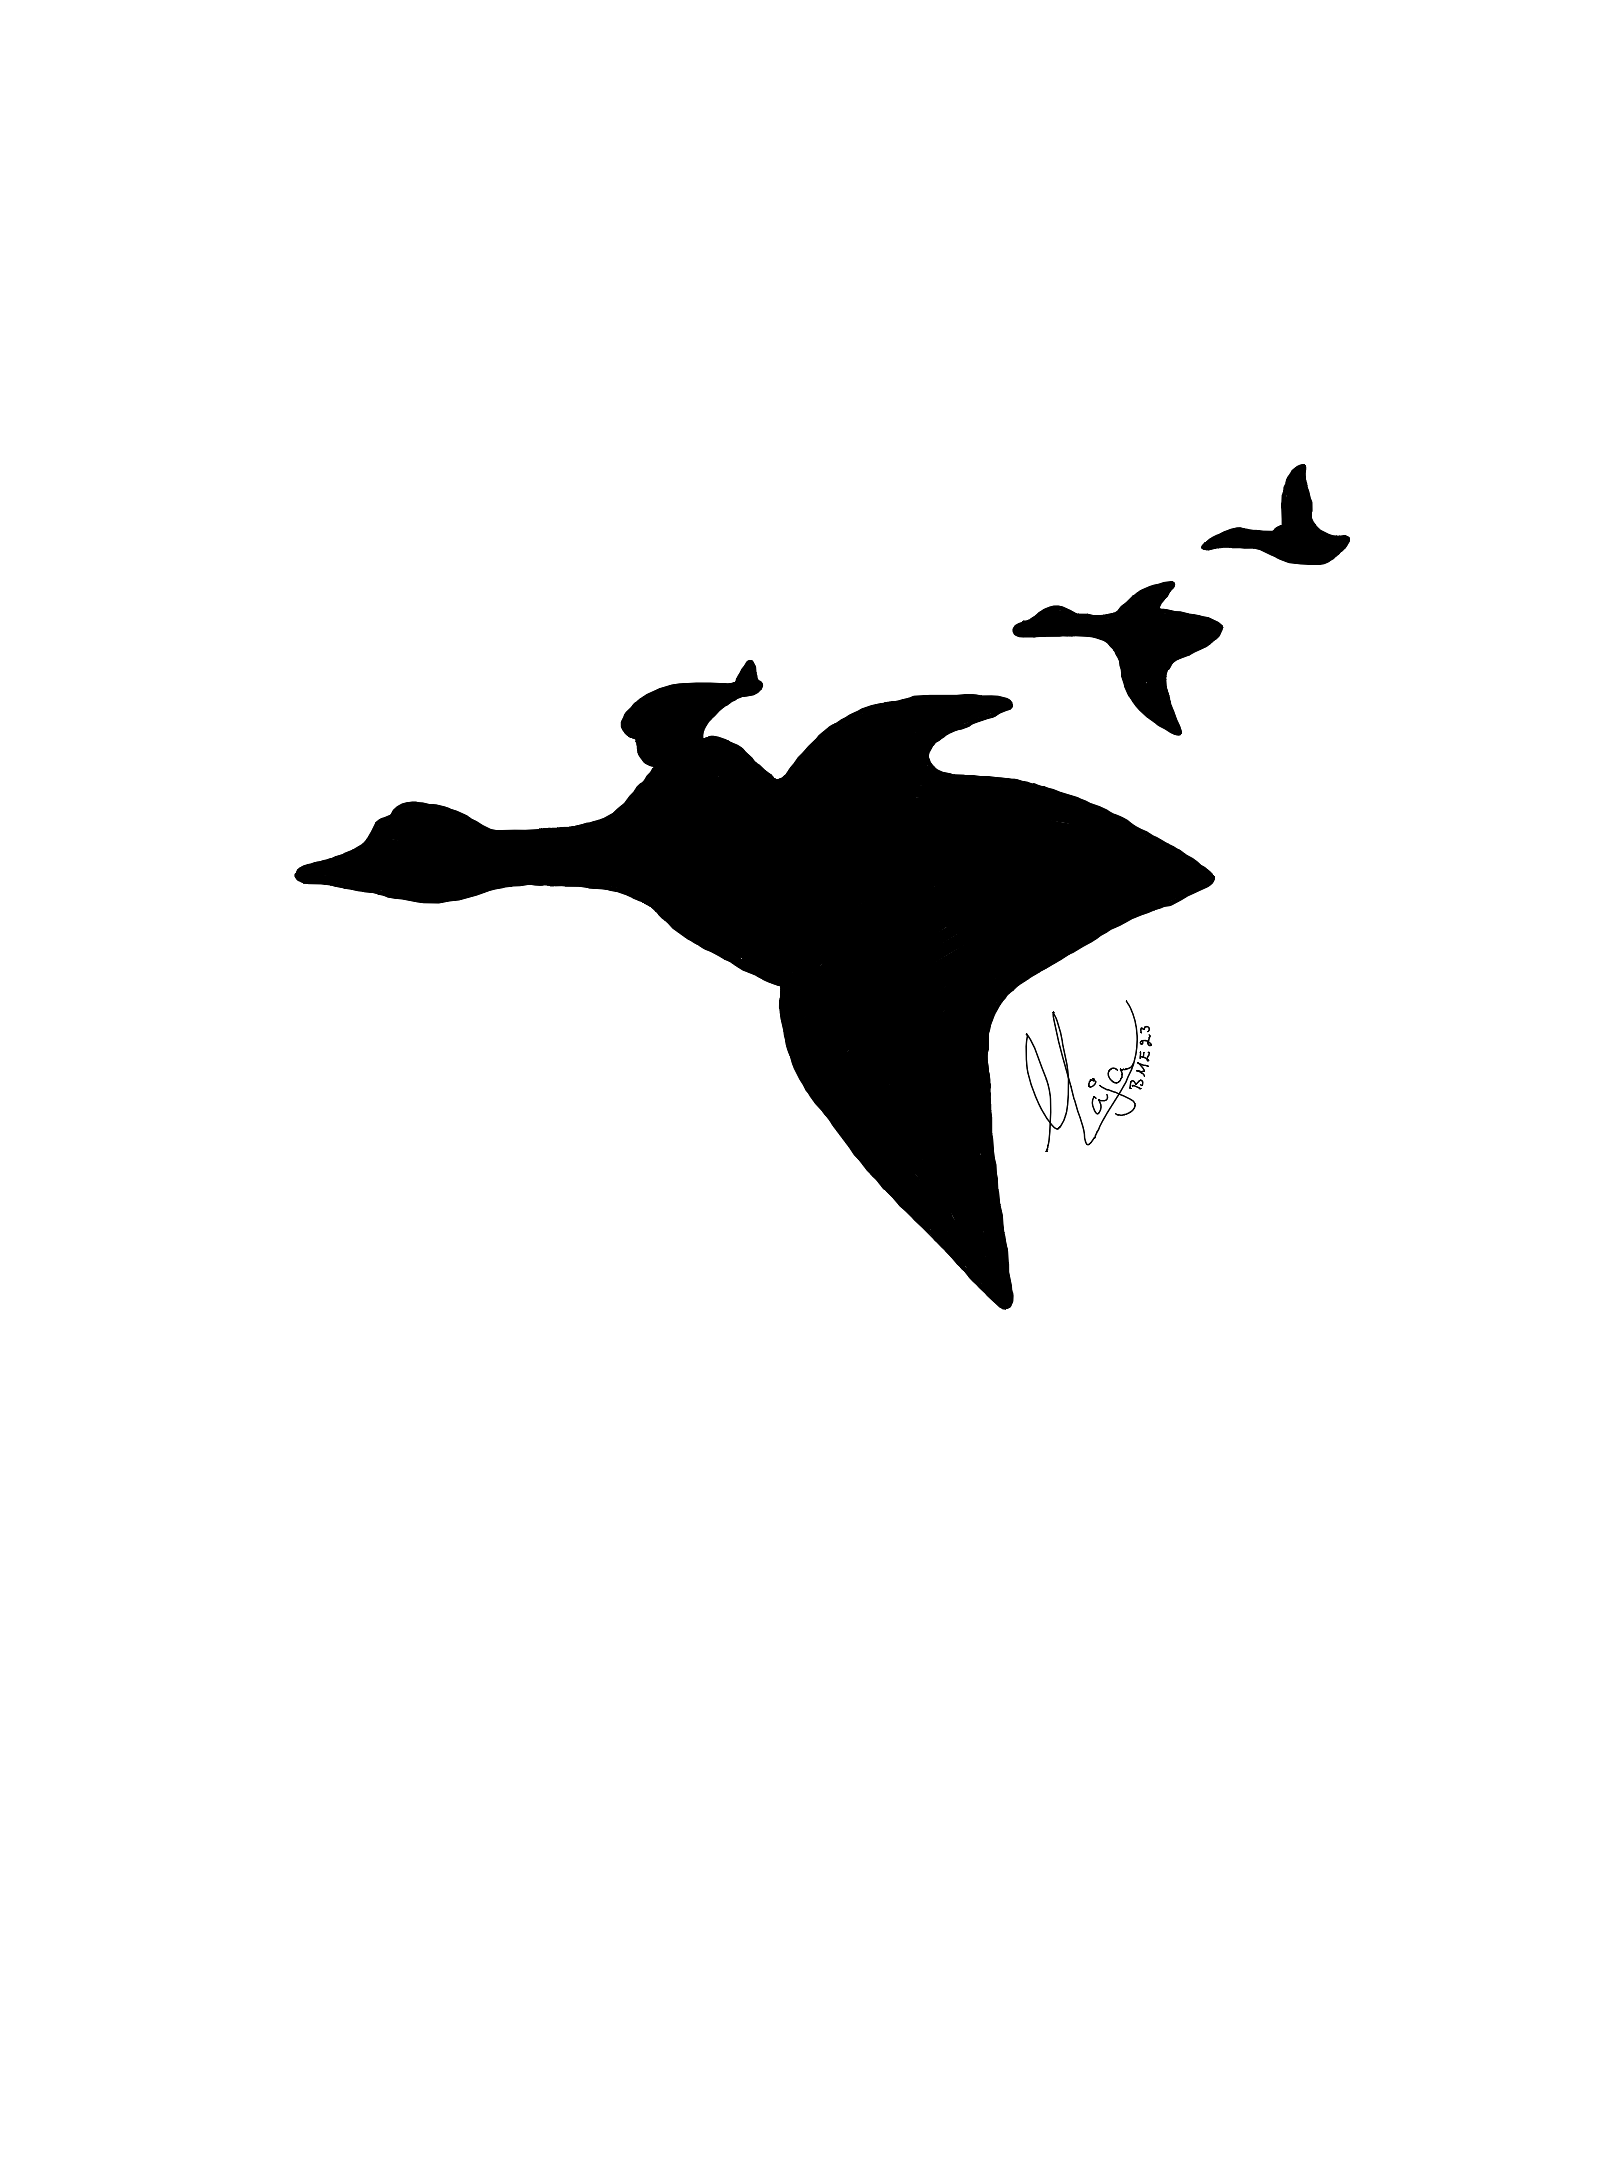
\includegraphics[width=6.5cm]{./bilder/majas-bilder/nils_holgersson.png}
% \end{textblock*}

\begin{textblock*}{3cm}(0.4cm,7.5cm) % {width}(x, y)
    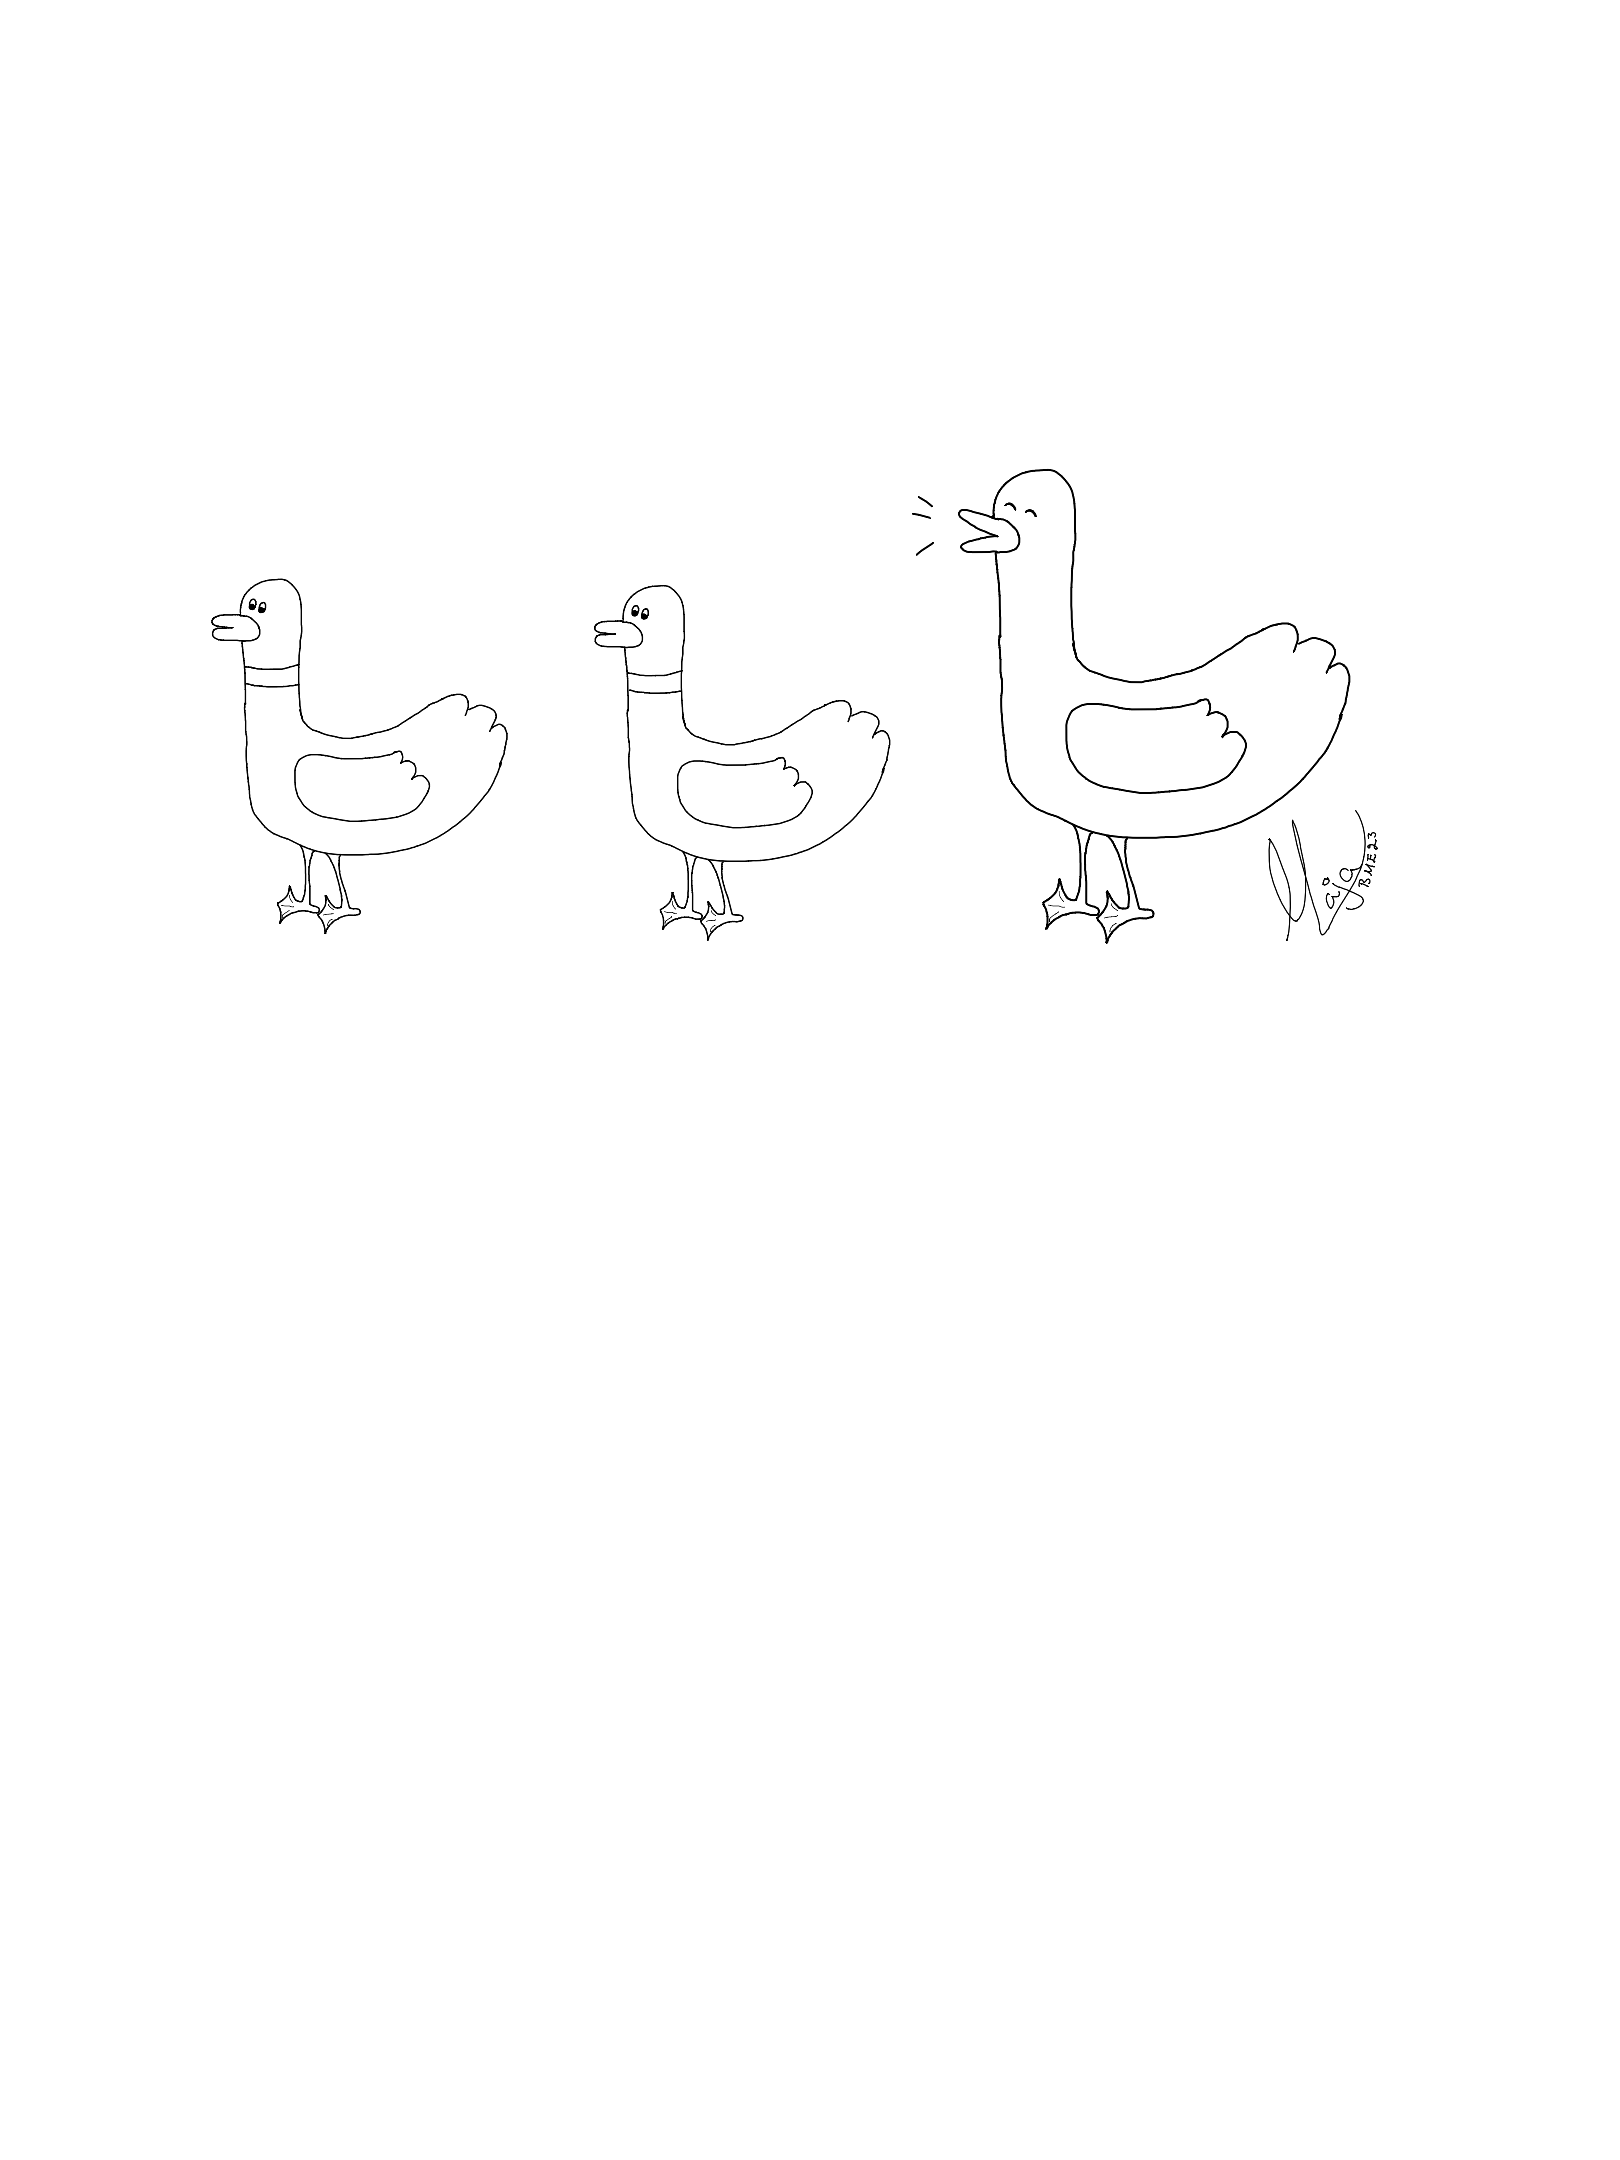
\includegraphics[width=10cm]{./bilder/majas-bilder/goose_utan_text.png}
\end{textblock*}

\begin{parse lines}[\noindent]{#1\\}
    Hela landet får njuta av vår akvavit
    Sockerbetan har lärt dom att dricka på bit
    Kan hända det retar en del,
    men i så fall är det deras eget fel
    Våran sandstrand den är både bländvit och fin
    och så har vi ju vår lilla vita kanin
    ||: Så låt dem... :||
    % Så låt dom bara gå på...

    Selma Lagerlöv som är en fin gammal dam,
    med Nils Holgersson gjorde för Skåne reklam
    Kan hända det retar en del,
    men i så fall är det deras eget fel
    % Kan hända det retar…
    Tänk sån nytta som storken från Skåne har gjort,
    men det hindrar ju inte att folk pratar lort
    % Men låt dem bara gå på vi klarar oss nog ändå
    ||: Så låt dem... :||
\end{parse lines}

\vissteduatt{Visste du att denna visa med fördel sjunges på grov skånska?}

\newpage
\resetBackground

\subsection*{Landskrona} 
\index[alfa]{Landskrona}
\index[anfa]{I Landskrona}
\songinfo{Mel: In the Ghetto}

\begin{parse lines}[\noindent]{#1\\}
    På en regnig strand
    Längs Skånes gråa västra kust 
    Bor några tusen fast dom inte har lust
    I Landskrona
    (I Landskrona)
    
    Flytta gärna dit
    Våran utsikt den är ganska käck
    Om man bortser ifrån Barsebäck
    Och det gör man
    (Inte riktigt)
    
    På krogen varje fredagskväll
    Där hänger Per och Kjäll
    Två fruktade lynniga bröder ifrån Ven
    
    Det är en kille ifrån Höör som stör
    Han har snott deras rullebör
    Nu ska dom ge han vad han tål med rör av rostfritt stål
    
    Sicket tufft klimat
    Men det finns en sak som förenar oss 
    Det är stadens stolthet BoIS förstås
    Heja svartvitt
    (Heja svartvitt)
\end{parse lines}

\newpage

\begin{parse lines}[\noindent]{#1\\}
    Att spela boll är kul
    På Landskrona IP står ett randigt gäng
    Dom har än en gång fått rejält med däng
    I Landskrona
    (Utav Mjellby)
    
    Sånna dagar känns det skit att va landskronit
    Vill ta pågatåget bort från stan
    Men på just den dan kan man ge sig fan
    På att det är strejk
    
    Så man vandrar hem en kulen kväll
    Och man träffar Kjell som åkt på en smäll
    Så han blör
    (Jäkla Höör)
    
    Men de ger aldrig upp
    För nästa helg tar vi nya tag
    Både BoIS och Per och Kjell och jag
    I Landskrona
    (I Landskrona)
\end{parse lines}

\newpage

\subsection*{Lite grann från ovan} 
\index[alfa]{Lite grann från ovan}
\index[anfa]{Jag är en liten gåsapåg från Skåne}
\songinfo{Text: Lasse Dahlqvist\\
Sång: Edvard Persson}

\begin{parse lines}[\noindent]{#1\\}
    Jag är en liten gåsapåg från Skåne
    En skåning som ni vet är alltid trygg
    Och fast jag är så nära sol och måne
    Jag sitter säkert på min gåsarygg
    Långt under mig det ligger som en tavla
    Det vackraste i världen man kan se
    Både skogar, sjö och strand
    Blir ett enda sagoland
    När man ser det lite grann så här från ovan

    Där ligger gamla slott och härresäten
    Som minnen från den stolta tid som flytt
    Och aldrig skall den tiden bli förgäten
    Men inget slag skall stånda här på nytt
    Nej, dessa fält skall bära samma skördar
    Som de har gjort i sekelflydda dar
    Ja det är min liv och kniv
    Alla tiders perspektiv
    När man ser det lite grann så här från ovan
\end{parse lines}

\vissteduatt{Visste du att 2020 genomfördes nollEgasque via Zoom till följd\\
 av pandemin? E6 körde ut maten med bil.}

\newpage
\noBackground

\begin{textblock*}{3cm}(3.0cm,7.0cm) % {width}(x, y)
    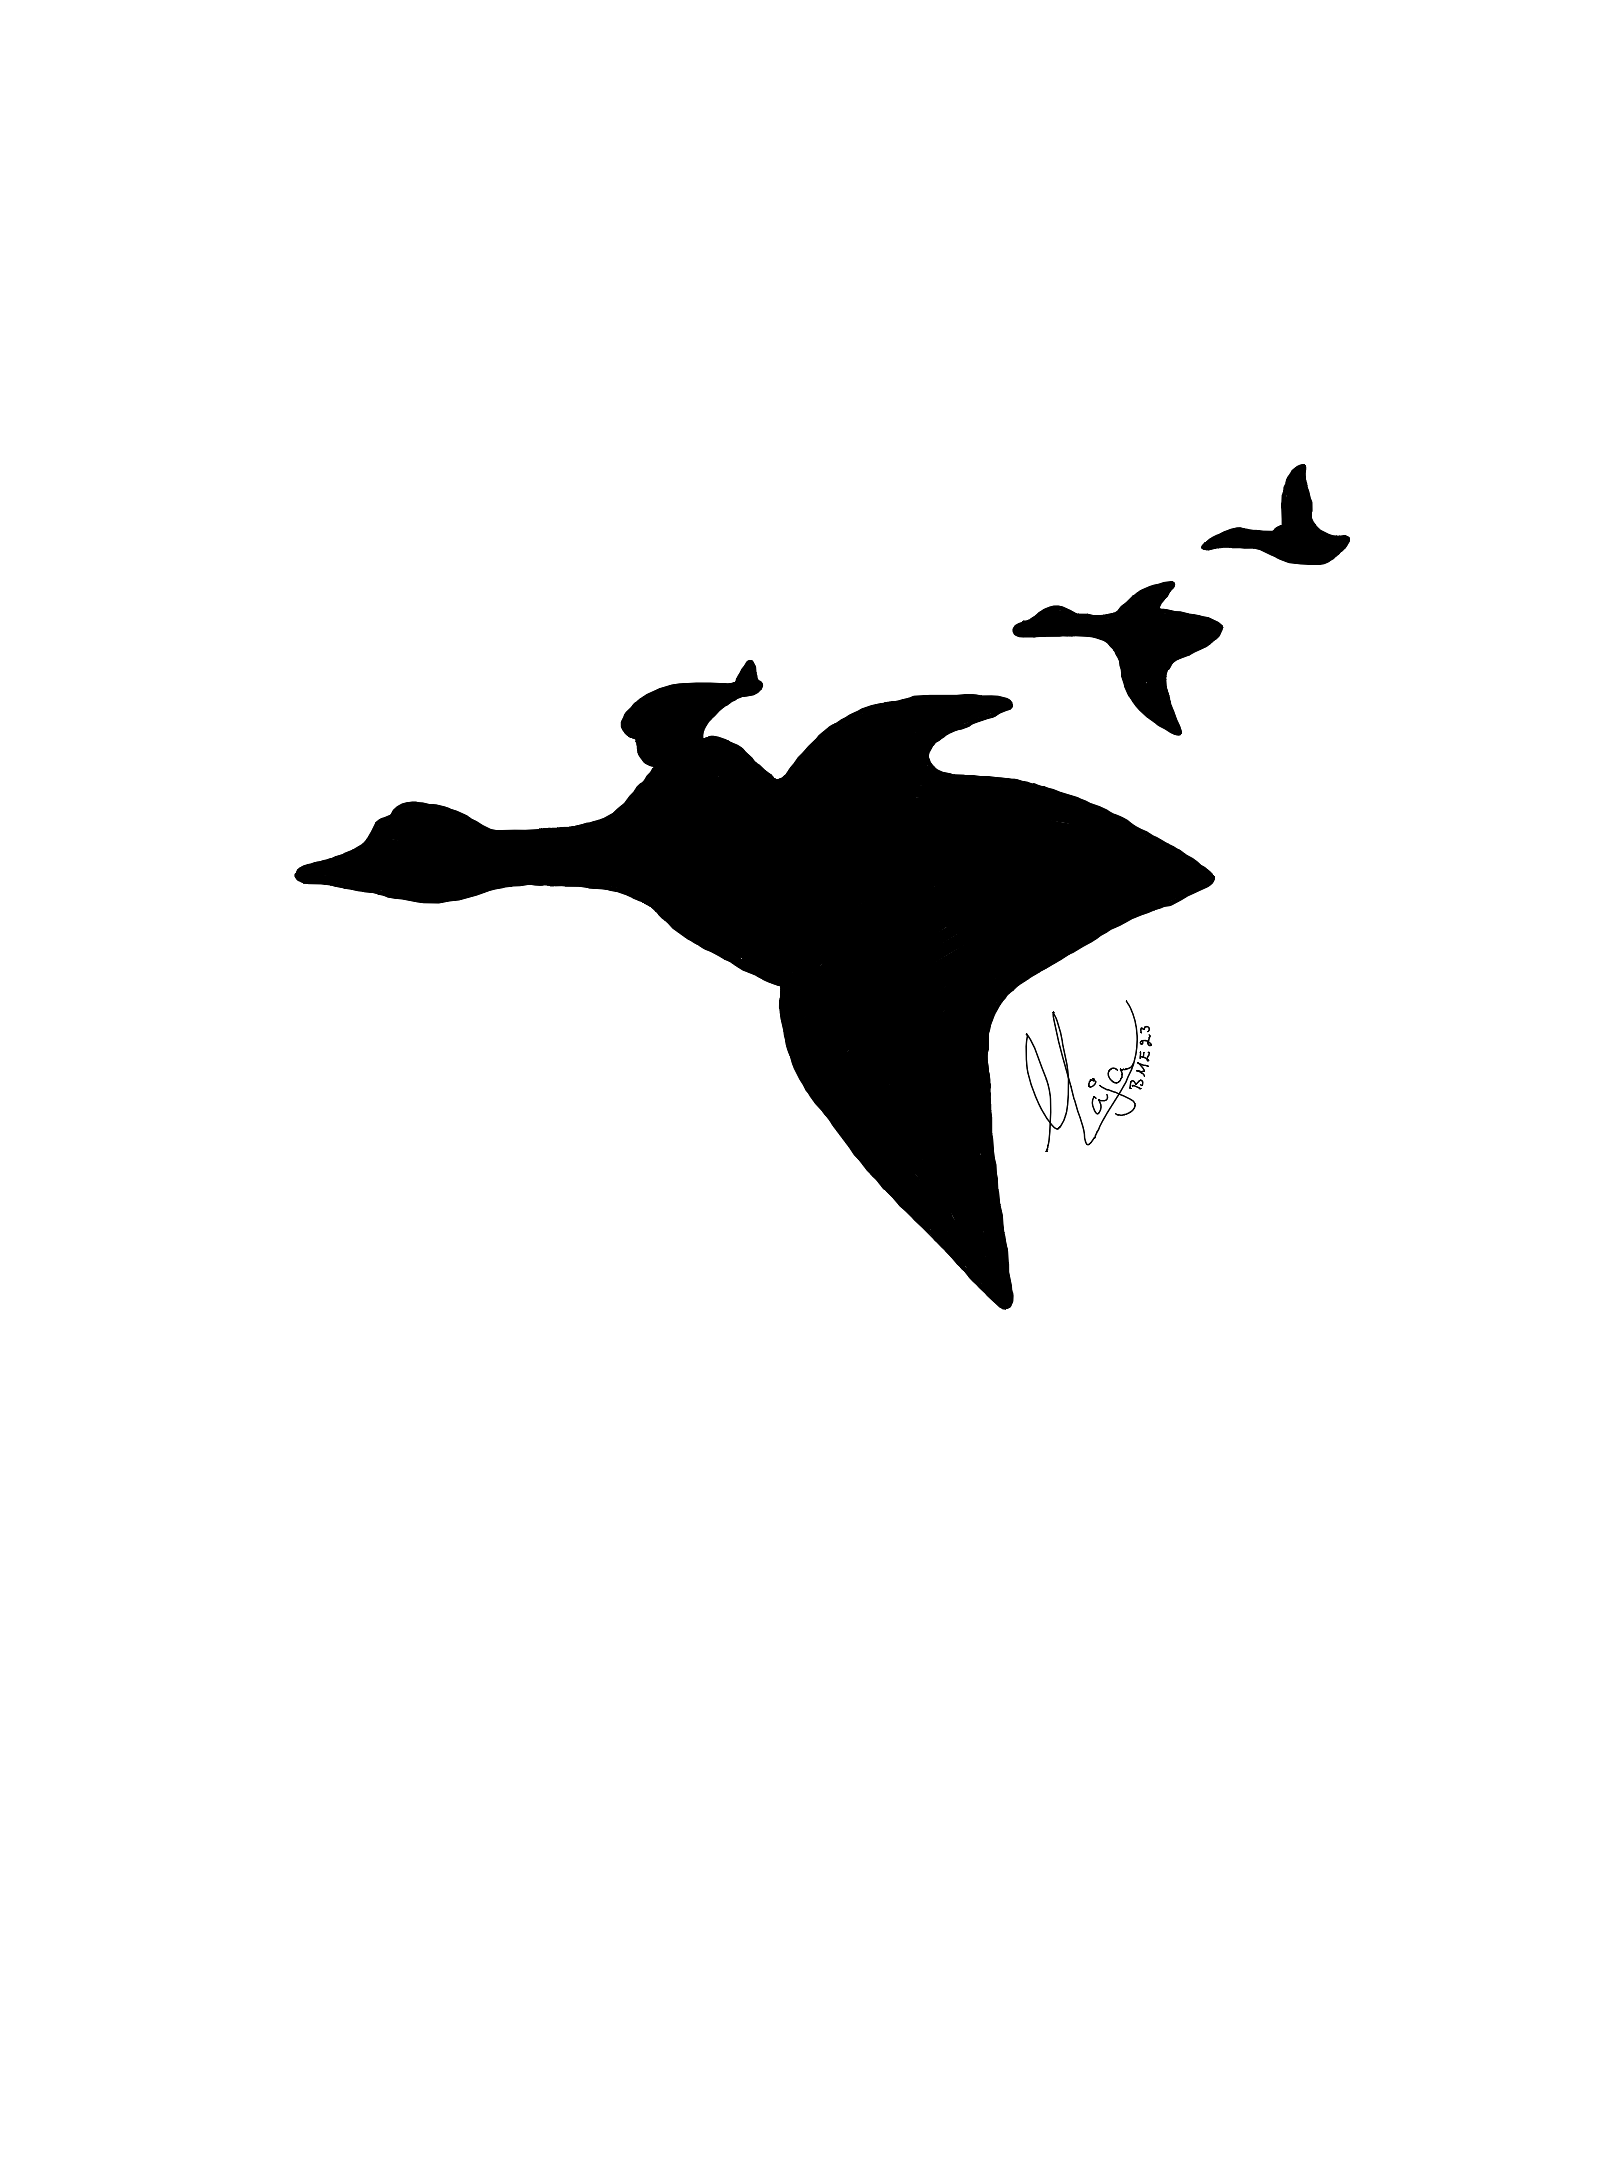
\includegraphics[width=7.5cm]{./bilder/majas-bilder/nils_holgersson.png}
\end{textblock*}

\begin{parse lines}[\noindent]{#1\\}
    Du kära gås som stolt i skyn dig svingar
    Har ingen farlig last att kasta ned
    Ty du bär fredens vita vackra vingar
    Som världen längtar efter mer och mer
    När människobarnen går därnere och kivas
    Då resonerar du nog liksom jag
    Tänk vad skönt det är ändå
    Att få sväva i det blå
    Och se er lite grann så här från ovan

    Nu jordens alla murar börjar skaka
    En samling dårar satt vår värld i brann
    Vad fäderna byggt upp blir pannekaka
    Det ryck och slits i gamla vänskapsband
    Ack kära ni som slåss därner på jorden
    Kom upp och ta en liten titt med mig
    Jag är ganska säker på
    Att ni skäms en smula då
    När ni ser vår gamla jord så här från ovan
\end{parse lines}

\vissteduatt{Visste du att 2021 genomfördes nollEgasque två gånger på \\
samma dag till följd av pandemin?}

\newpage 
\resetBackground

\subsection*{Skånsk madavisa} 
\index[alfa]{Skånsk madavisa}
\index[anfa]{Rabbemos å spegefläsk}
\songinfo{Mel: Aspelöv ock Lindelöv}

\begin{parse lines}[\noindent]{#1\\} 
Rabbemos å spegefläsk,
panntofflagröd med knudor,
fläskasvålar, grisatassar,
prinsakorv med snudor
Fittamadar, sillarumpor,
sylta med rödbedor,
äggakaga, revbensspjäll

Luad ål å rögad ål
å ål som di har halmad
Kogad ål å stegad ål
å ål i gelatin
Ålasluring, ålapudding
ål med chokeladsås,
rutten ål å ål i kål

Hussegröd å puggavälling,
kläggefläsk med bläror
Tösaflabbar, flinerumpor,
pattagris med päror
Glyttanäsor, hunnarövar,
lummemög med hylle,
mormor Karnas hönsafjös

Sillasupen, ålasupen,
supen till sardellen
Fläskasupen, rabbesupen,
suparna till spjällen
Gåsasupen, äggasupen,
suparna till supen
å till sist en kagesup

Spiddekaga, kransekaga,
flarn å mazariner,
sockerkaga, butterkaga
nötter å praliner
Risengröd med vispegrädde,
punsch å karameller
Sen e de' dags för nattamad!

\end{parse lines}

\subsection*{Eslövs nationalsång} 
\index[alfa]{Eslövs nationalsång}
\index[anfa]{Vi går här på slätten och vi hackar våra bedor}

\begin{parse lines}[\noindent]{#1\\}

    ||: Vi går här på slätten
    och vi hackar våra bedor
    Vi går här på slätten och hackar hela dan :||
    ||: Åååh, hackar våra bedor
    Åååh, hackar hela dan :||

    ||: Jag ska vända mig, och bocka mig,
    och ta en liten beda
    Jag ska vända mig, och bocka mig,
    och ta en beda till :||
    ||: Åååh, jag tar en liten beda
    Åååh, jag tar en beda till :||
\end{parse lines}

\vissteduatt{Vissde due add skeuåska aer ded feijnaste spraåked i hela \\
vaerlden?}
\newpage

\subsection*{Skåne} 
\index[alfa]{Skåne}
\index[anfa]{Nu har det blivit dags att dricka skåne}
\songinfo{Mel: Lite grann från ovan}

\begin{parse lines}[\noindent]{#1\\}
    Nu har det blivit dags att dricka Skåne
    En liten sträv, så gyllengul som raps
    Det är det bästa mellan sol och måne
    Som lätt får mången stark till snabb kollaps
    Så fatta nu din hand om hela Skåne
    Här kommer södra Sverige i en snaps
    Känn hur Lund och Smygehuk
    slår små volter i din buk
    Aquaviten ska va' gul
    och heta Skåne
\end{parse lines}


\subsection*{Till den skånska metropolen Vinslöv} 
\index[alfa]{Till den skånska metropolen Vinslöv}
\index[anfa]{Vinslöv}
\songinfo{Mel: Wiensk operettvals}

\begin{parse lines}[\noindent]{#1\\}
    I vin, i vin, i vin, i vin,
    i Vinslöv bor min mor
    På Hven, på Hven, på Hven, på Hven,
    påven han bor i Rom
    I Rom, i Rom, i Rom, i Rom,
    i rompan på en ko
    I ko, i ko, i ko, i ko,
    i Kosta göra man glas
    I glas, i glas, i glas, i glas,
    i glas där har man vin
    I vin, i vin, i vin, i vin,
    i Vinslöv bor min mor
\end{parse lines}

\vissteduatt{Visste du att fler snapsvisor finns på sida 108?}
\newpage
%\vspace*{-4cm}
\enlargethispage{5cm}
%\vspace*{3.6cm}
\subsection*{Skånska slott och herresäten} 
\index[alfa]{Skånska slott och herresäten}
\index[anfa]{På himmelen vandra sol, stjärnor och måne}
\songinfo{Text: Hjalmar Gullberg \& Bengt Hjelmqvist\\
Sång: Edvard Persson}

\begin{parse lines}[\noindent]{#1\\}
    På himmelen vandra sol, stjärnor och måne
    Och kasta sitt fagraste ljus över Skåne
    På höga och låga, på stort och på smått
    På statarens koja och ädlingens slott

    Se månstrålen in genom blyrutan faller
    Och tecknar på golvet det järnsmidda galler
    Stolts jungfrun hon drömmer i majnattens ljus
    Att friare komma till Glimmingehus

    På utflykt till bokskogen malmöbon glor upp
    Mot raden av strålande fönster på Torup
    Att smaka på kaka som bakats på spett
    Dig ber hennes nåd, friherrinnan Coyet

    Där rådjuren skymta bak'vitgråa stammar
    Man ser Toppela'gård med broar och dammar
    Systemet på sprit och på skatterna sta'n
    Där lurar belåtet fiskalen Aschan

    Med port genom huset och gamla kanaler
    Lyss Skabersjö ännu till jaktens signaler
    Själv kungen i nåder far dit från sitt slott
    Och skjuter fasaner med grevarna Thott

    Och därefter hälsar han på baron Trolle
    Och jagar och spelar sin sans och sin nolle
    Allt medan baronens gemål
    Plockar gräs åt rastupp och rashöna på Trollenäs
\end{parse lines}
\newpage